% !TEX root = main.tex

\section{Optimal Control of Pitch/Travel with Feedback (LQ)}
\subsection{LQR}
In the previous exercise we calculated the optimal path, and fed it to the PID controllers. This worked well, but when the helicopter reached the final position, it did not stay there, as it did not correct for the drift in position due to momentum and differences in the propellers. This can be corrected with the use of a second controller between the optimization layer and the basic control layer. This controller will ensure that the helicopter stays on the planned trajectory.

This second regulator is implemented as a LQ controller. This regulator minimizes the cost function $J$ defined by

\begin{equation}
    J = \sum^{\infty}_{i=0} \mathbf{\Delta} \mathbf{x}^T_{i+1}\mathbf{Q}\mathbf{\Delta} \mathbf{x}_{i+1}+\mathbf{\Delta} \mathbf{u}_i^T R \mathbf{\Delta} \mathbf{u}_i
\end{equation}

The $\mathbf{Q}$ and $R$ was chosen to be

\begin{subequations}
    \begin{align}
        \mathbf{Q} &= \begin{bmatrix}
            50 & 0 & 0 & 0\\
            0 & 1 & 0 & 0 \\
            0 & 0 & 10 & 0\\
            0 & 0 & 0 & 10
        \end{bmatrix}\\
        R &= 1
    \end{align}
\end{subequations}

Using these weights we implemented the LQ controller using the code found in listing \ref{lst:LQ} and the simulink diagram found in \cref{fig:simulink_LQ}.

\begin{lstlisting}[caption={MatLab code for LQ controller},label=lst:LQ]
    Q = diag([50 1 10 10]);
    R = diag(1);

    [K,S,e] = dlqr(A1, B1,Q,R);
\end{lstlisting}

\begin{figure}
    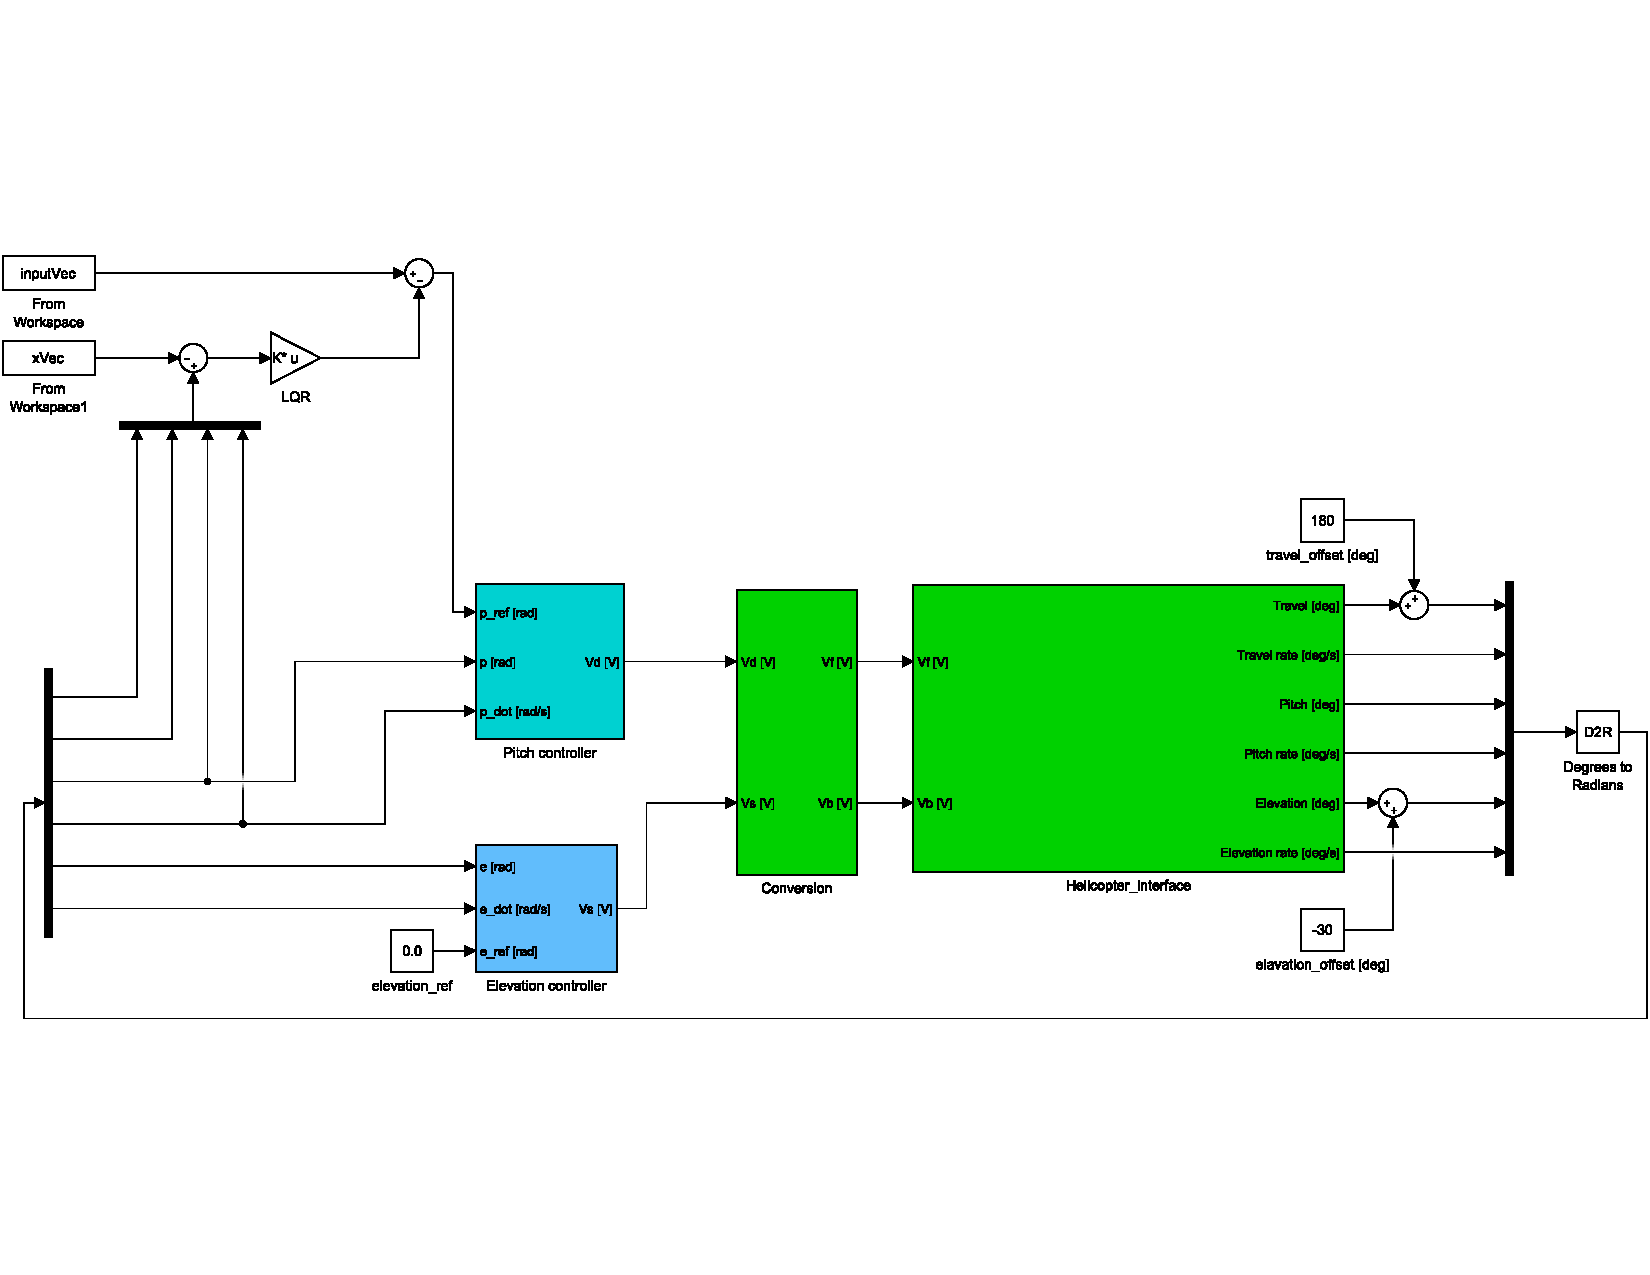
\includegraphics[width=\textwidth]{ex3sim.pdf}
    \caption{Simulink diagram including LQ controller}
    \label{fig:simulink_LQ}
\end{figure}

\begin{figure}
    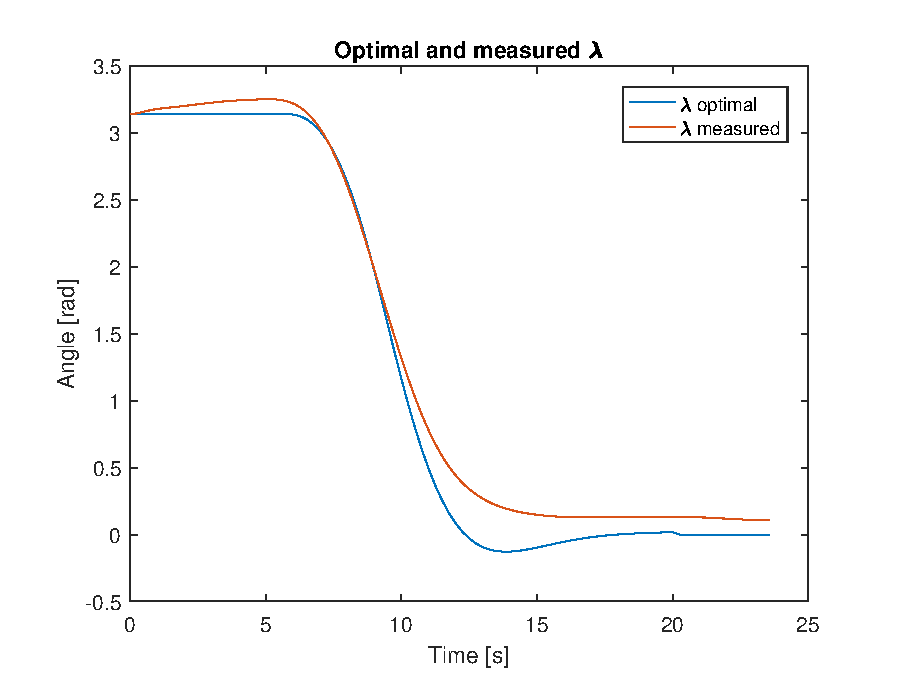
\includegraphics{optimal_and_measured_lambda_ex3.eps}
    \caption{Optimal and measured $\lambda$ with feedback (LQ)}
    \label{fig:opt_meas_lambda_ex3}
\end{figure}

This gives us the response seen in \cref{fig:opt_meas_lambda_ex3}. As we can see, we no longer have the drifting problem experienced earlier. We do, however have a constant error. This error could be removed if the LQ controller also had an integral term.

\subsection{MPC}
MPC can be realized by solving a finite horizon open loop optimal control problem at each time step. This calculates the optimal trajectory from the current position at each timestep, then applies the first input. In this way the MPC implement sa feedback loop, and finds the optimal way to cancel out disturbances. This is computationally expensive, but you get the ability to add constraints, a feature lacking in simpler controllers. A consequence of this is that while we have to use three layers of control, one to find the optimal trajectory, one to ensure that the helicopter stays on the trajectory and one to control the acuators, a MPC combines the first two layers, and as such only needs two layers. 

%\todo[inline]{Skriv om de neste to avsnittene så de blir sanne}
%
%One advantage with MPC compared to LQR is that MPC is more robust. This is because the MPC calculates a new optimal input for each timestep, rather than doing everything a priori. In addition, MPC allows the use of constraints.
%
%On the other hand, MPC is far more resource-demanding than LQR. Also, the solution using MPC is usually not optimal in the context of the cost function (as mentioned above, it optimizes with respect to stability or other metrics). Another downside to MPC is that it requires a model of the system, while LQR does not.
